\chapter{Reverberation Mapping Analysis of NGC4593}
\label{cap: Results}

\section{Line Determination}

Having obtained the AVG- and RMS spectrum of NGC4593, the next step is the identification of the emission lines. Figure \ref{fig:AVG_RMS_SPECTRUM} and \ref{fig:UV_uncalibrated_AVG_RMS} show the optical to near-infrared range between $3900 \AA$ and $9000 \AA$ and  the UV range between $1100 \AA$ and $1700 \AA$, respectively. 

\begin{figure}[!htbp]
	\centering
	\makebox[\textwidth][c]{%
		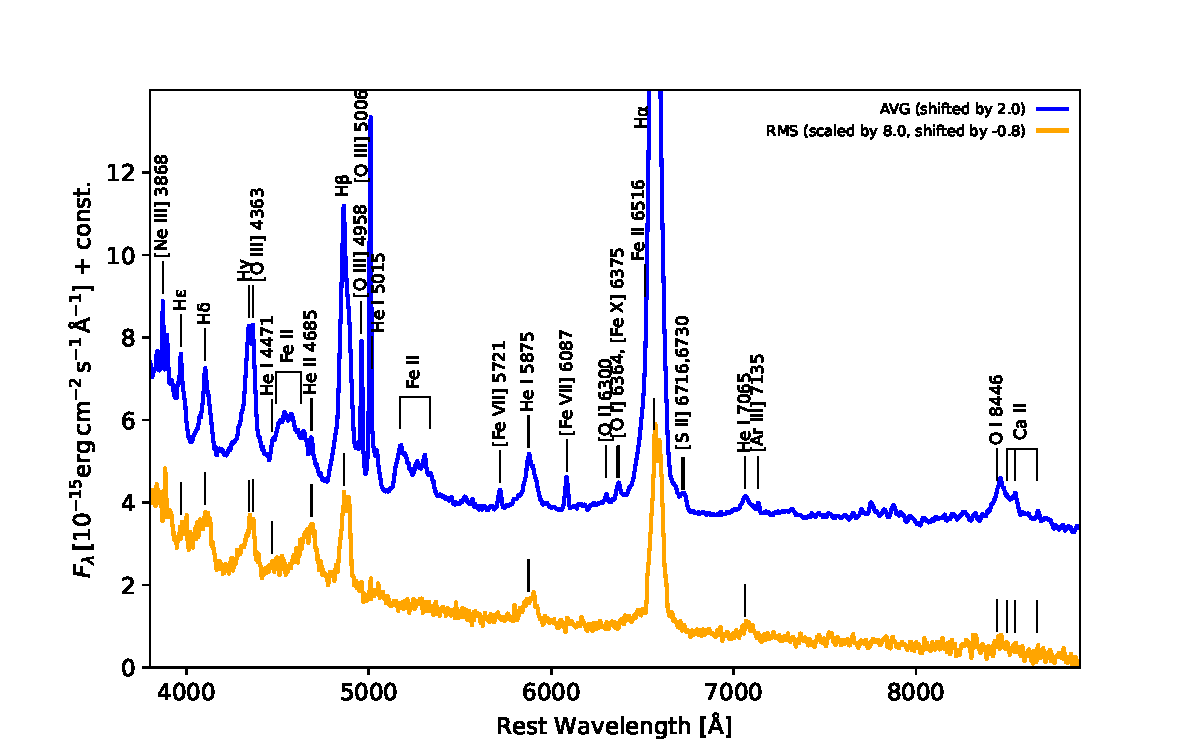
\includegraphics[width=1.2\textwidth]{pictures/Chapter4/avg_rms_spec/avg_rms_spec.pdf}}
	\caption{Optical AVG and RMS spectrum with determined emission lines.}
	\label{fig:AVG_RMS_SPECTRUM}
\end{figure}

\newpage

Looking at Figure \ref{fig:AVG_RMS_SPECTRUM}, the most prominent broad emission lines in the AVG spectrum are the Balmer-Lines, with H$_\alpha$ being the strongest followed by $H_\beta$ and $H_\gamma$. Their variations are clearly visible in the RMS spectrum and the line profiles of H$_\alpha$ and H$\beta$ in particular show strong similarities, which will be discussed in more detail later in this chapter. In addition to the Balmer emission lines there are several He-emission lines such as He\,II $\lambda 4685$, He\,I $\lambda 5875$ and He\,I $\lambda 7065$ show measurable variability. Another significant broad emission line complex appears in the far-red part of the spectrum, including the O\,I $\lambda 8446$ and Ca\,II lines. The O\,I $\lambda 8446$ line is of particular interest in this thesis, as it shows variation which was never measured through a reverberation mapping analysis before. \\
Apart from the broad emission lines, the AVG spectrum also exhibits several strong forbidden emission lines with the [O\,III] $\lambda 5007$ and the [O\,III] $\lambda 4958$ as the most prominent ones. As mentioned in the previous chapter, the first one was used for the intercalibration of the spectra and, as expected, shows no variability in the RMS spectrum, similar to the other forbidden lines. Finally, the AVG spectrum shows additionally two Fe II emission line groups, that shows no variation in the RMS spectrum.

\begin{figure}[!htbp]
	\centering
	\makebox[\textwidth][c]{%
		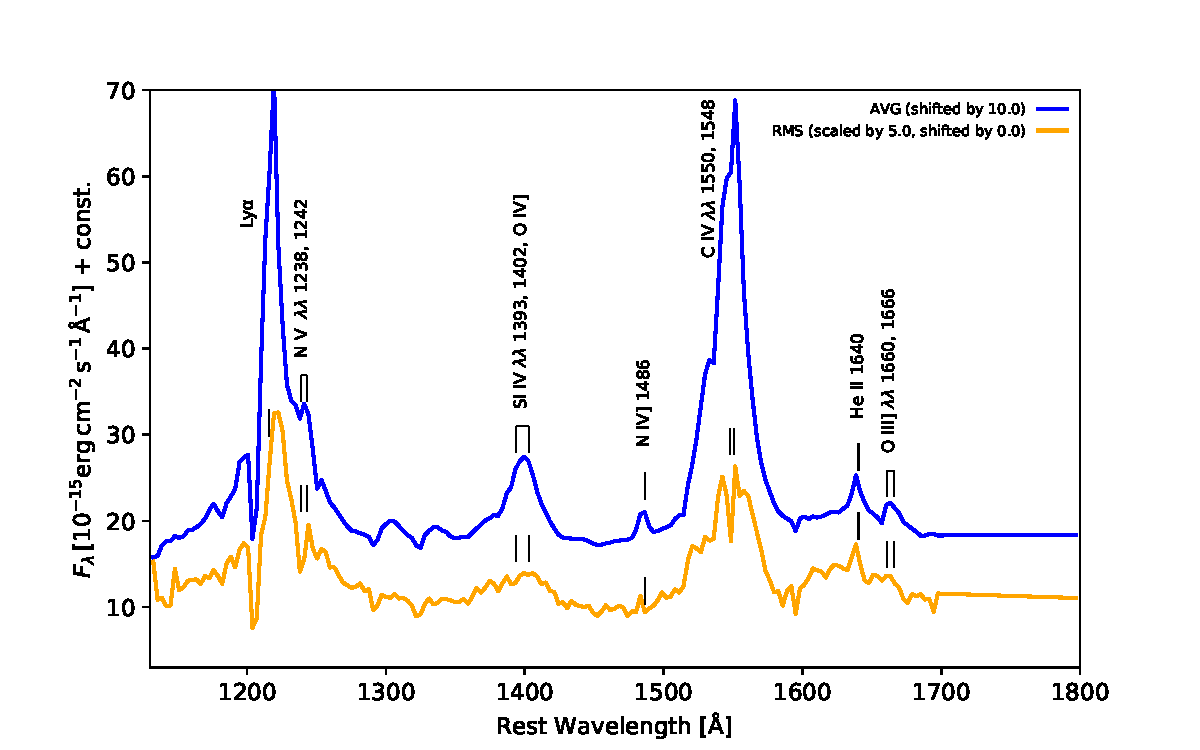
\includegraphics[width=1.2\textwidth]{pictures/Chapter4/avg_rms_spec/UV_uncalibrated_AVG_RMS.pdf}}
	\caption{UV spectrum AVG and RMS spectrum with determined emission lines}
	\label{fig:UV_uncalibrated_AVG_RMS}
\end{figure}


The UV spectrum, shown in figure \ref{fig:UV_uncalibrated_AVG_RMS}, contains only a few additional broad and semi-forbidden emission lines due to its limited coverage. In addition to the prominent Si and C broad emission lines, it shows strong and variable Ly$_\alpha$ emission, which is of particular significance for this thesis. \\
The Bowen fluorescence of O\,I $\lambda 8446$, which is investigated in this analysis, is typical driven by the emission of the Ly$_\beta$ line, which lies outside the spectral range of the HST Campaign. However, as can be seen in figure \ref{fig:UV_uncalibrated_AVG_RMS}, Ly$_\alpha$  still lies in the spectral range of the campaign, as the most blue broad line of the taken spectra. As Ly$_\alpha$ and Ly$_\beta$ are assumed to originate from the same physical region, Ly$_\alpha$ can be used to examine the correlation of O\,I $\lambda 8446$ and Ly$_\alpha$ for Bowen fluorescence.
 
 




\section{Emission Line and Continua Measurement}

After identifying the emission lines, the next step of the analysis is to calculate the fluxes of those lines. This is done by integrating the flux density over the extent of each emission line for every observed spectrum of the campaign. Here it is important to define the integration limits so that only the variable component of the emission line is measured in this way. To ensure this, a parallel view of the AVG- and RMS-spectrum was used to define those integration limits, by identifying the variable components of the line in the RMS-spectrum. Additionally, it must be ensured, that no component of any other line is contributing to the line flux of the measured line, which can lead to misleading conclusions. But before the line flux can be calculated, the surrounding continuum has to be subtracted, which can be done by interpolating a linear pseudo-continuum between sections on the blue and red side with no line contribution. The chosen integration limits and pseudo-continua can be found in Table \ref{tab:emission_lines}. With the fluxes of each line now derived from all observed spectra, it is possible to extract the lightcurves and variability statistics of the measured emission line, which will be further covered in the next section.\\
Besides the emission line lightcurves, continua lightcurves from different wavelength ranges are needed for the further analysis. The extraction process is similar to the emission line lightcurves, except that they get calculated by the mean flux density of a sufficiently large region without line emission or absorption. Logically a pseudo-continua subtraction is not needed here. The chosen integration limits for the continua can be found in Table \ref{tab:continua}.



\begin{table}[h!]
	\centering
	\small
	\caption{Integration Limits and Pseudo-Continua of the measured emission lines}
	\label{tab:emission_lines}
	\begin{tabular}{lcc}
		\hline
		\hline
		\textbf{Line} & \textbf{Integration Limits} & \textbf{Pseudo-Continua}  \\
		\hline
		Ly$_\alpha$ & $1207-1238$ & $1151-1161, 1462-1468$\\
		NV$\,\lambda 1238$ & $1238-1274$ & $1151-1161, 1461-1468$ \\
		SiIV$\,\lambda 1393$ & $1359-1423$ & $1151-1161, 1461-1468$ \\
		CIV$\,\lambda 1548$ & $1511-1579$ & $1461-1468, 1679-1686$ \\
		HeII$\,\lambda 1640$& $1599-1644$ & $1461-1468, 1679-1686$ \\
		\hline
		H$_\alpha$ & $6520-6634$ & $6107-6129, 6861-6900$ \\
		H$_\beta$ & $4828-4924$ & $4762-4774, 5085-5112$ \\
		H$_\gamma$ & $4317-4391$ & $4197-4220, 4435-4450$ \\
		H$_\delta$ & $4065-4153$ & $4026-4033, 4197-4220$ \\
		
		HeI$\,\lambda5875$ & $5840-5941$ & $5645-5653, 6044-6057$ \\
		HeII$\,\lambda4685$ & $4610-4744$ & $4435-4450, 4762-4774$ \\
		OI$\,\lambda 8446$ & $8380-8498$ & $8005-8031, 8850-8955$ \\
		\hline
		OIII$\,\lambda 5007$ & $4982-5033$ & $4762-4774, 5085-5112$ \\
		\hline
		\hline
	\end{tabular}
\end{table}

\begin{table}[h!]
	\centering
	\small
	\caption{Integration Limits of the measured continua}
	\label{tab:continua}
	\begin{tabular}{lc}
		\hline
		\hline
		\textbf{Line} & \textbf{Integration Limits}  \\
		\hline
		Cont. 1150 & $1151-1161$\\
		Cont. 1460 & $1458-1472$\\
		Cont. 4010 & $4026-4033$\\
		Cont. 4200 & $4192-4220$\\
		Cont. 4440 & $4435-4450$\\
		Cont. 4765 & $4762-4774$\\
		Cont. 5100 & $5085-5112$\\
		Cont. 5600 & $5645-5653$\\
		Cont. 6045 & $6044-6057$\\
		Cont. 6110 & $6107-6129$\\
		Cont. 6880 & $6861-6900$\\
		Cont. 7390 & $7382-7405$\\
		Cont. 8015 & $8005-8031$\\
		Cont. 8900 & $8864-8955$\\
		\hline
		\hline
	\end{tabular}
\end{table}




\section{Lightcurves}
...
\subsection{Continua}
...
\begin{figure}[!ht]
	\centering
	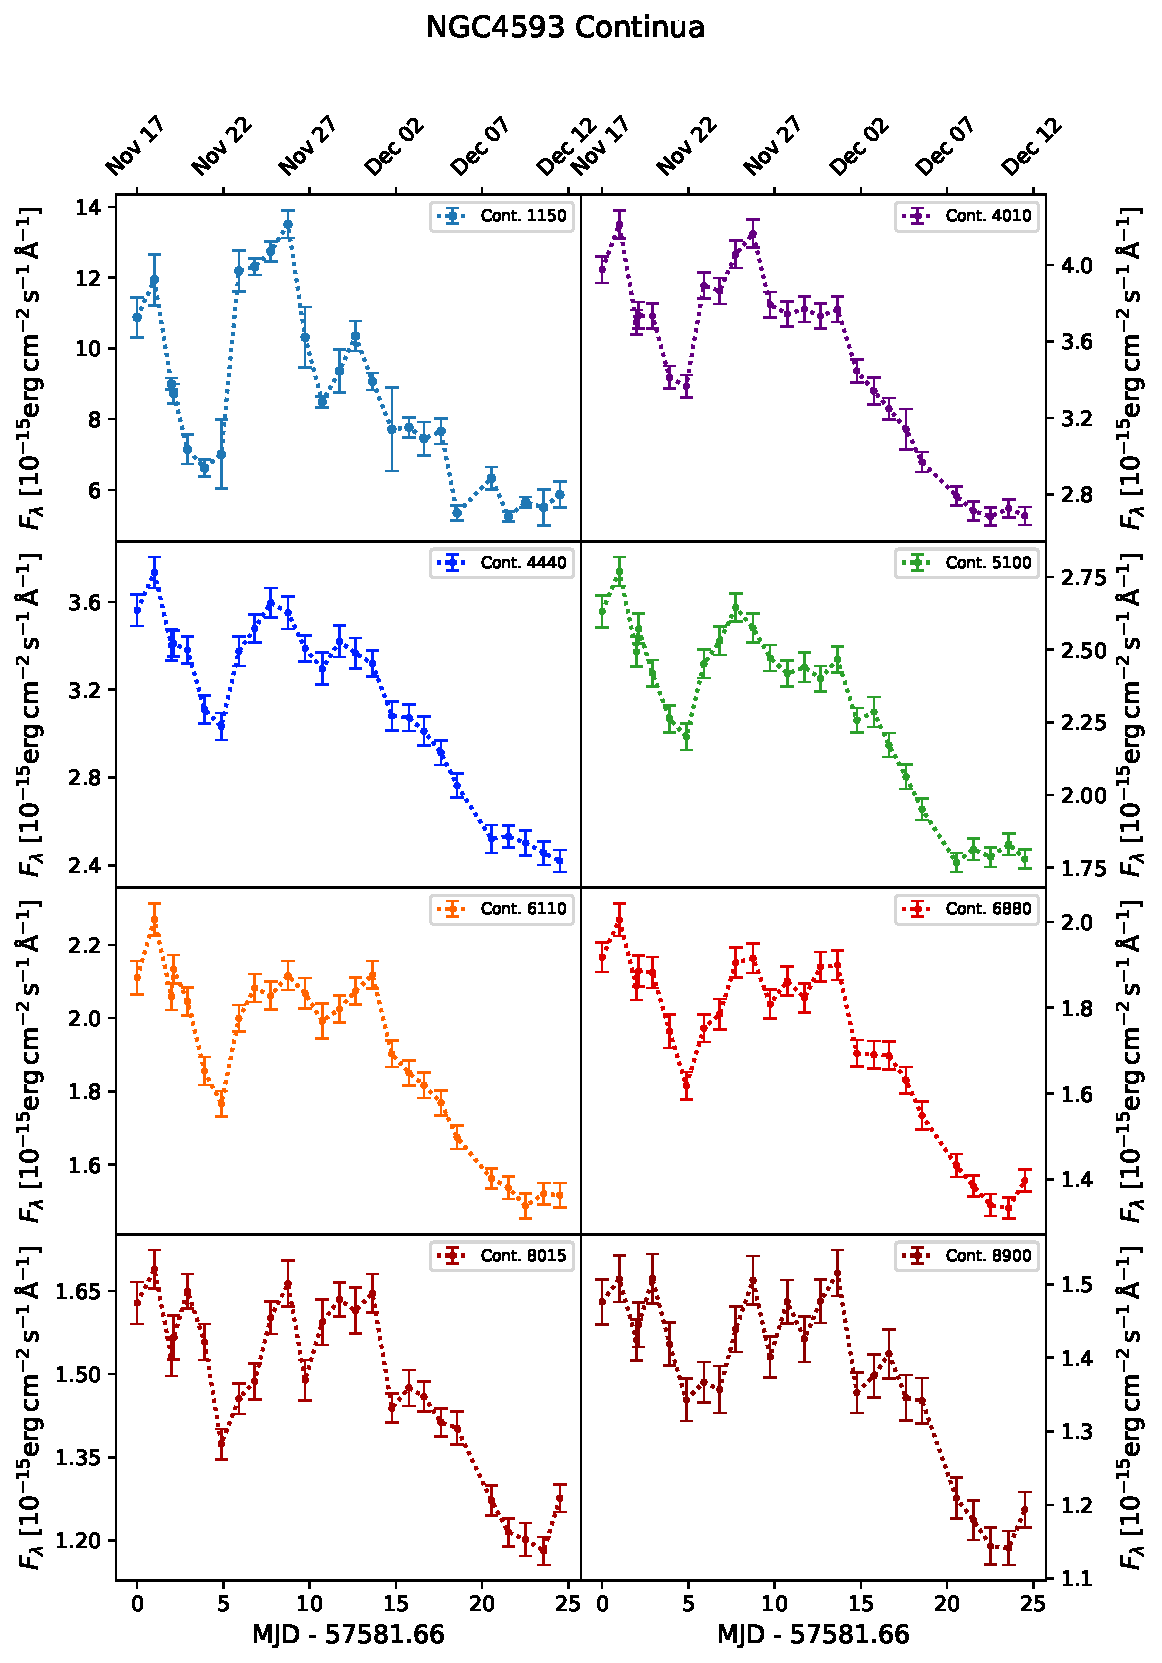
\includegraphics[width=0.9\textwidth]{pictures/Chapter4/lightcurves/NGC4593_Continua.pdf}
	\caption{...}
	\label{fig:continua_lightcurves}
\end{figure}

\subsection{Emission Lines}
...
\begin{figure}[!ht]
	\centering
	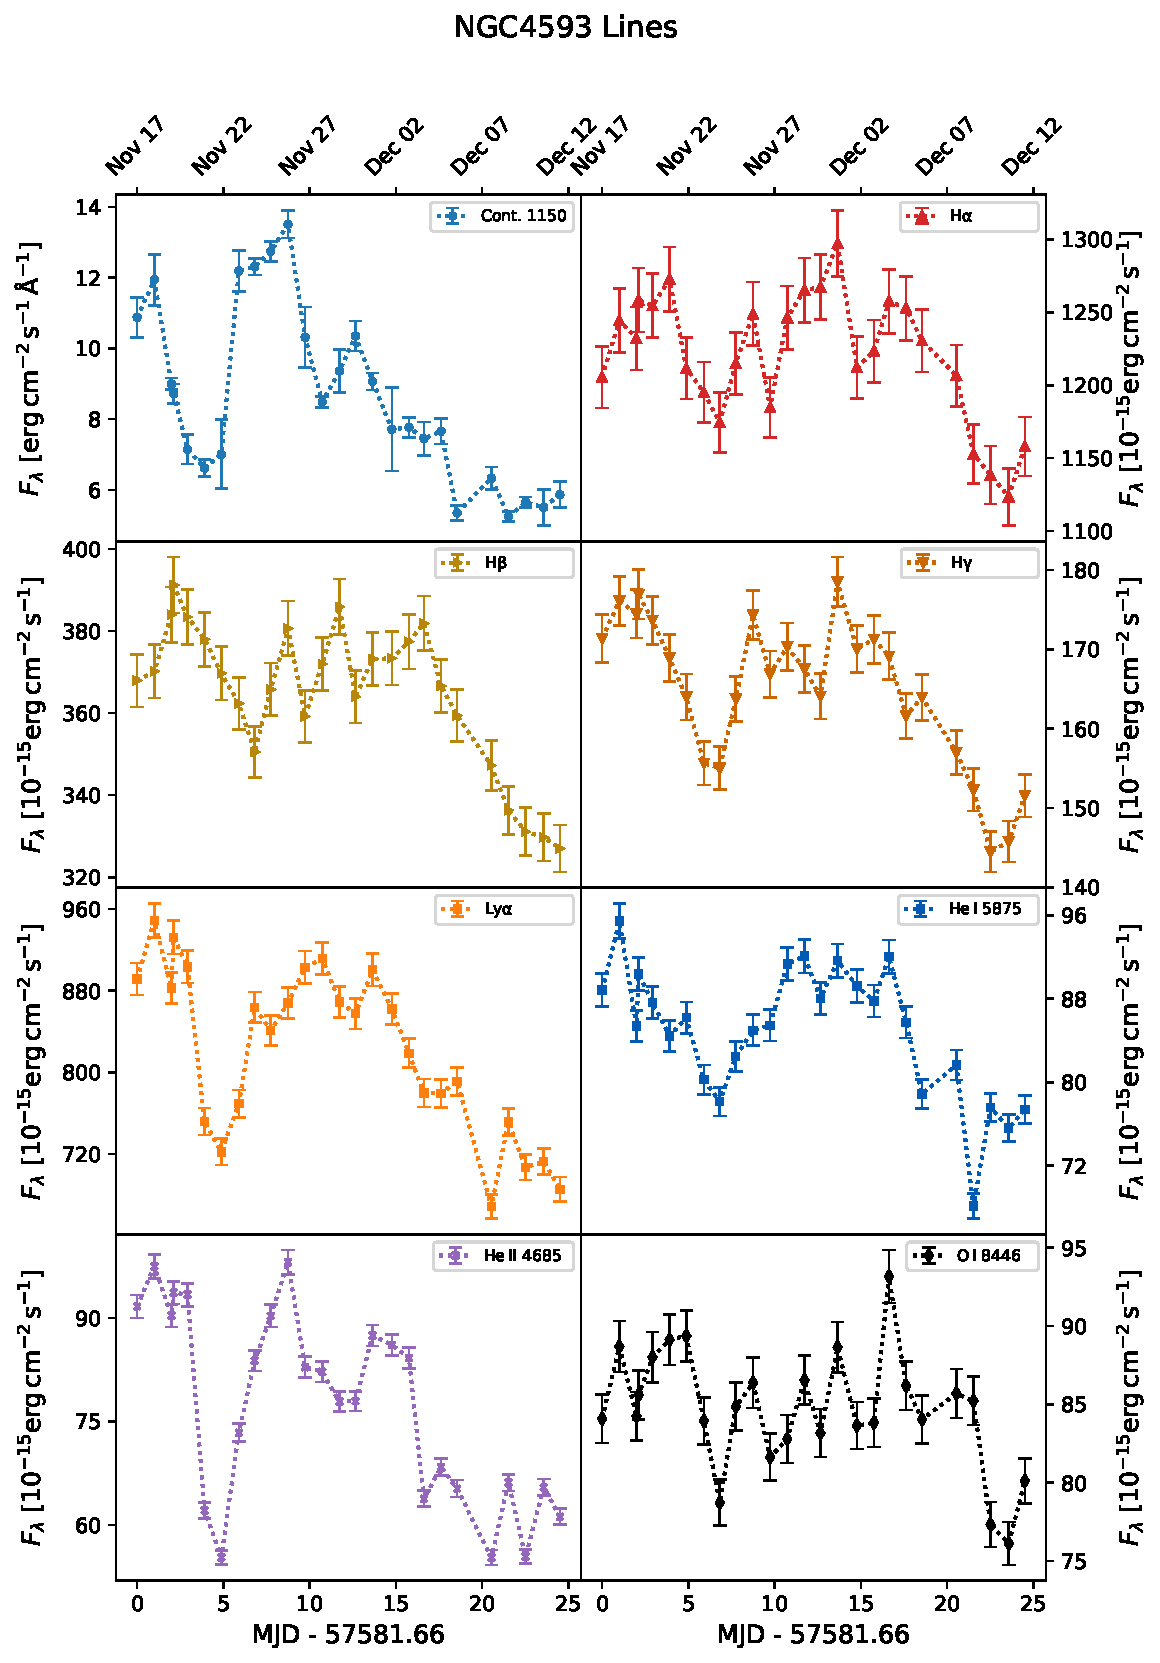
\includegraphics[width=0.9\textwidth]{pictures/Chapter4/lightcurves/NGC4593_Lines.pdf}
	\caption{AVG RMS Spektrum}
	\label{fig:emission_line_lightcurves}
\end{figure}

\section{Line Profiles}

\begin{figure}[!ht]
	\centering
	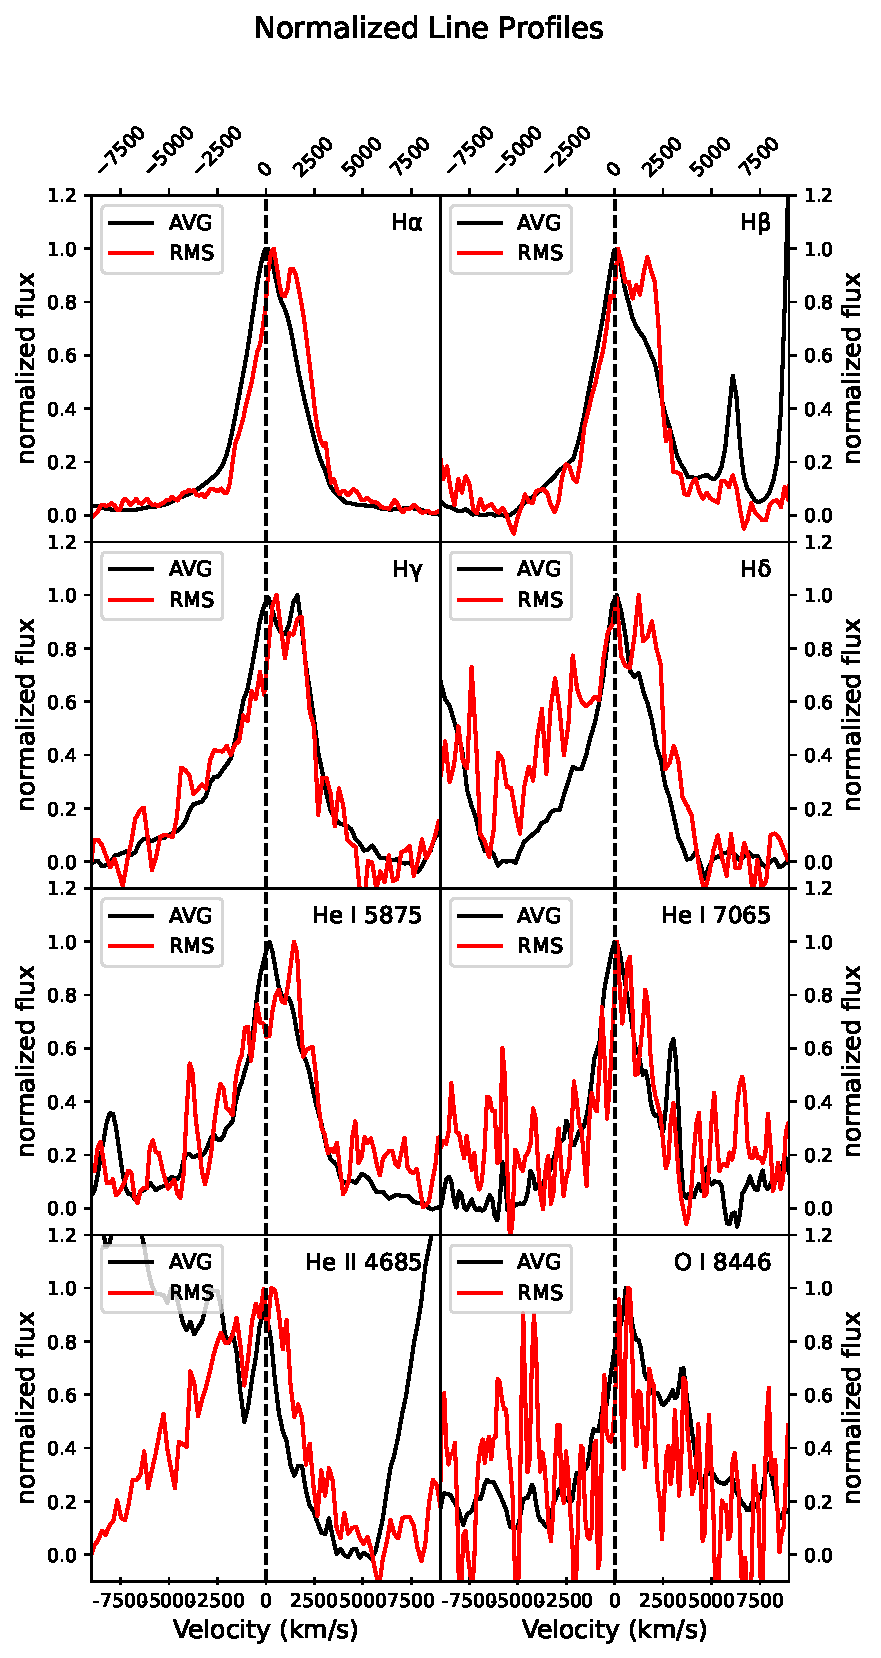
\includegraphics[width=0.8\textwidth]{pictures/Chapter4/line_profiles/Normalized_Line_Profiles.pdf}
	\caption{AVG RMS Spektrum}
	\label{fig:line_profiles}
\end{figure}

\section{Time Lag and BH Masses}

\begin{figure}[!ht]
	\centering
	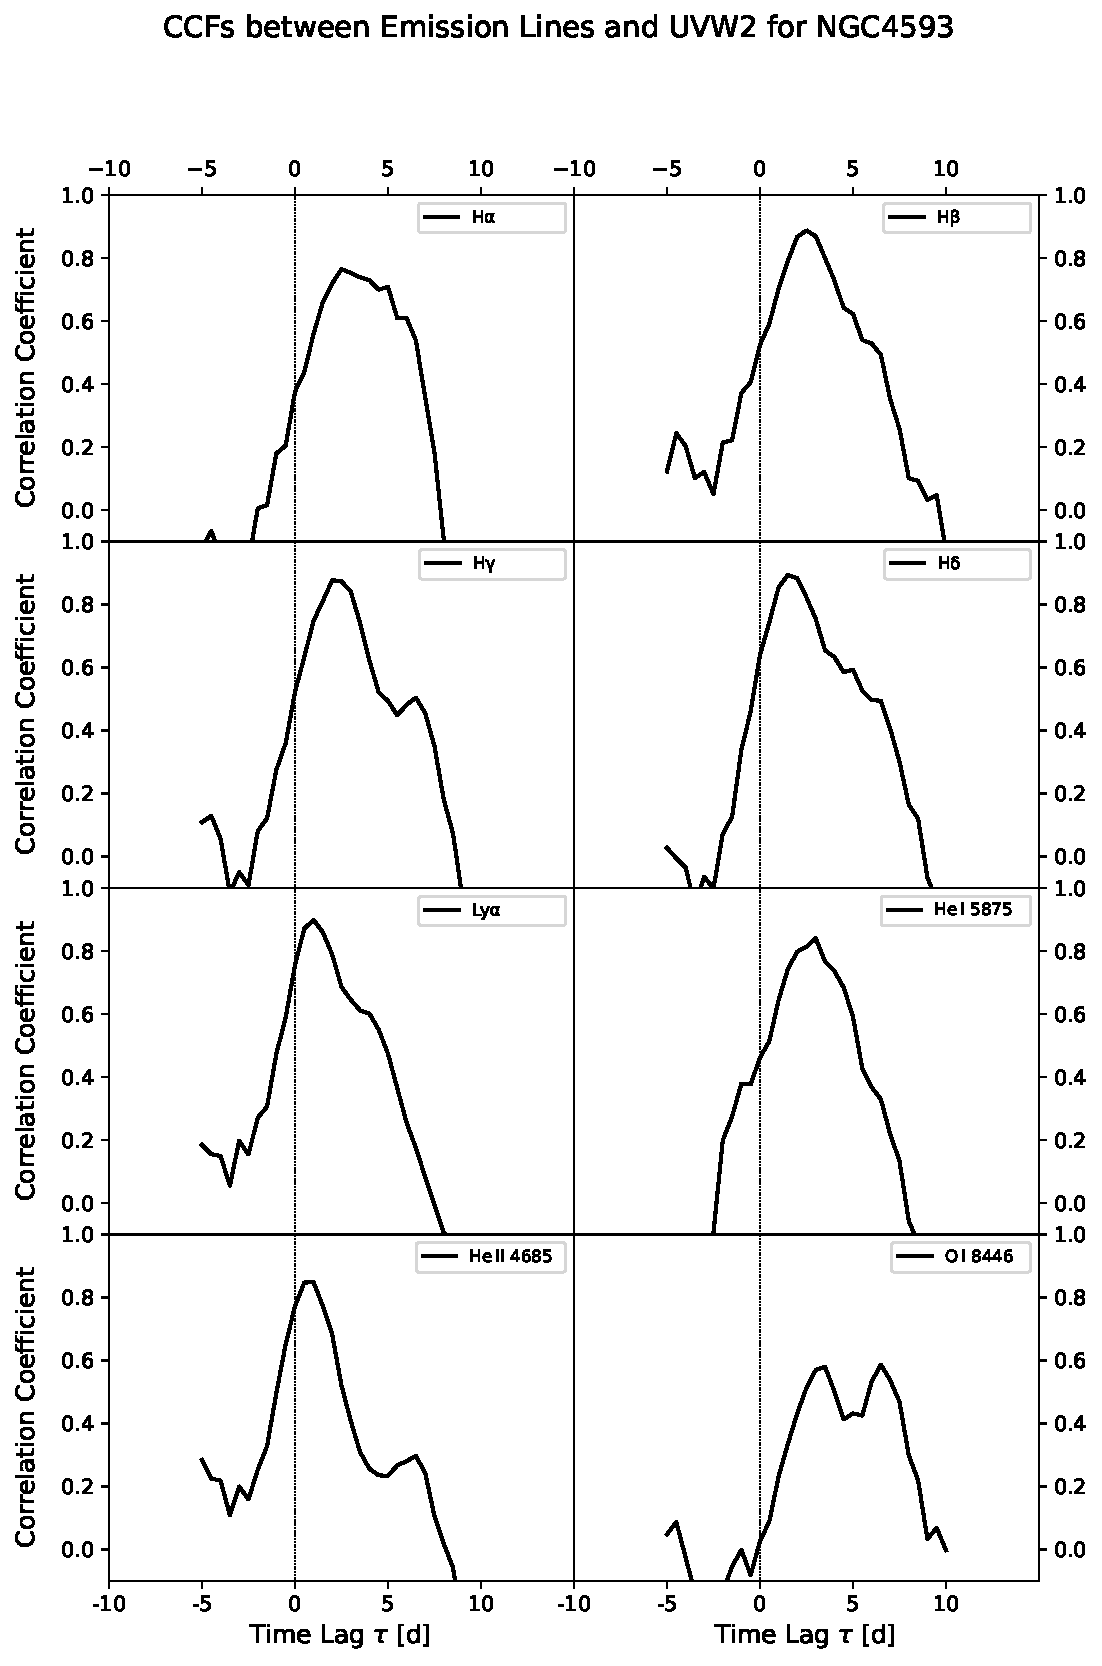
\includegraphics[width=0.9\textwidth]{pictures/Chapter4/ccfs/CCFs_H_He_LyA_O_UVW2.pdf}
	\caption{AVG RMS Spektrum}
	\label{fig:ccfs}
\end{figure}

\begin{figure}[!ht]
	\centering
	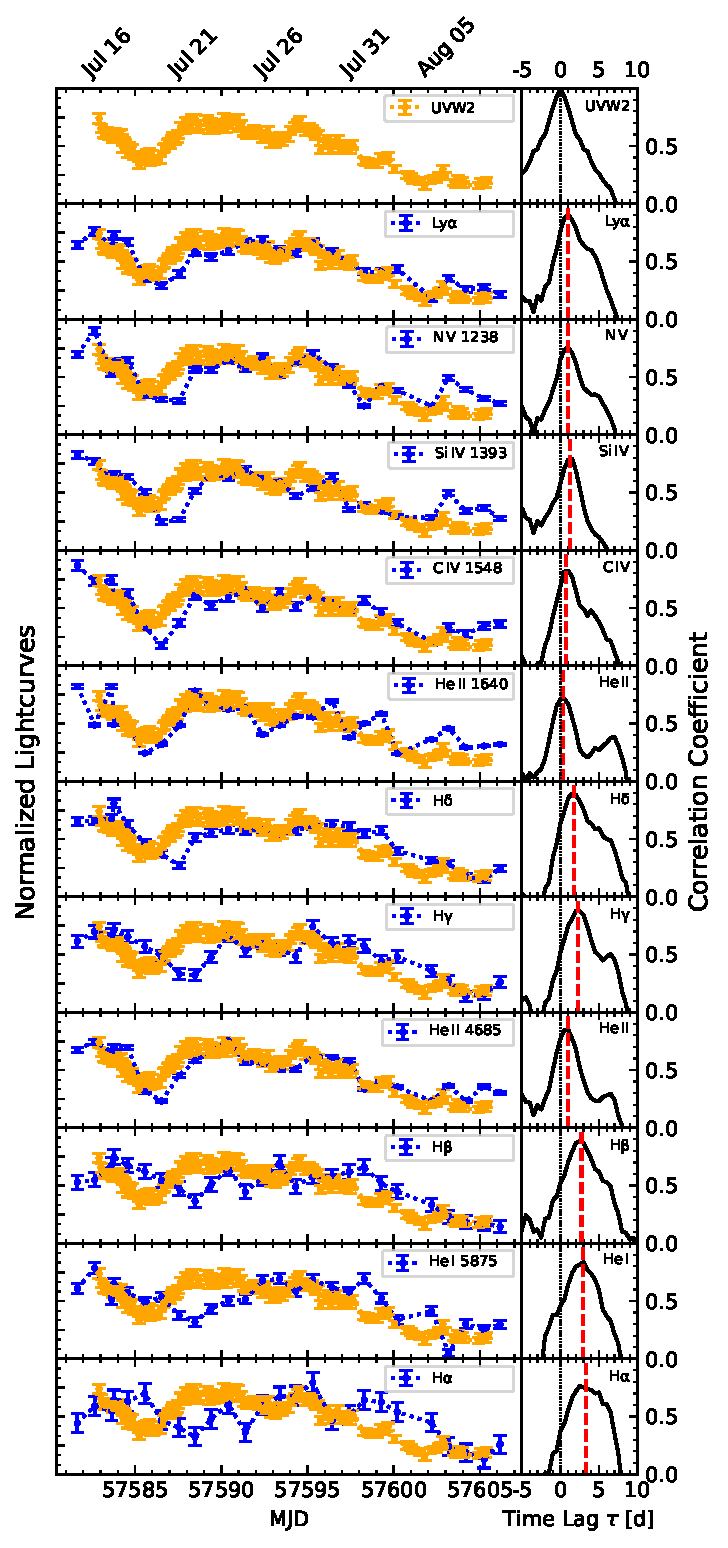
\includegraphics[width=0.7\textwidth]{pictures/Chapter4/lighcurves_and_ccfs_and_time_lag_tables/UV_to_HAlpha_ccfs_and_reference_lightcurves.pdf}
	\caption{AVG RMS Spektrum}
	\label{fig:ccfs_lightcurves}
\end{figure}

\section{Bowen Fluorescence}